% !TEX root = ../main/main.tex
\section{Results and discussion}
 
 \begin{figure}[h]
 \begin{subfigure}[t] {0.23\textwidth}
 \centering
 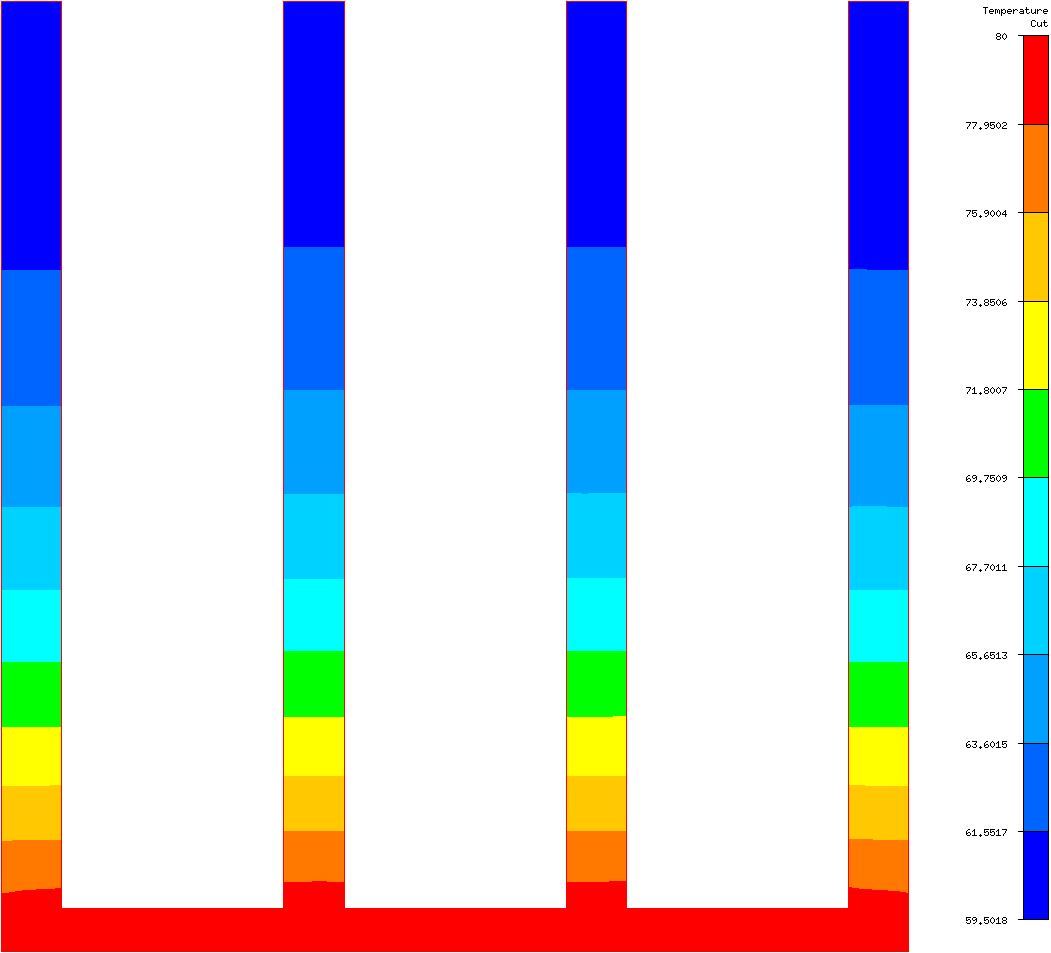
\includegraphics[width=0.7\textwidth]{../figures/heatsink4_h105_gmf005.png}
 \caption{"Placeholder"}
 \label{fig:res_4_1}
 \end{subfigure}
 ~
  \begin{subfigure}[t] {0.23\textwidth}
 \centering
 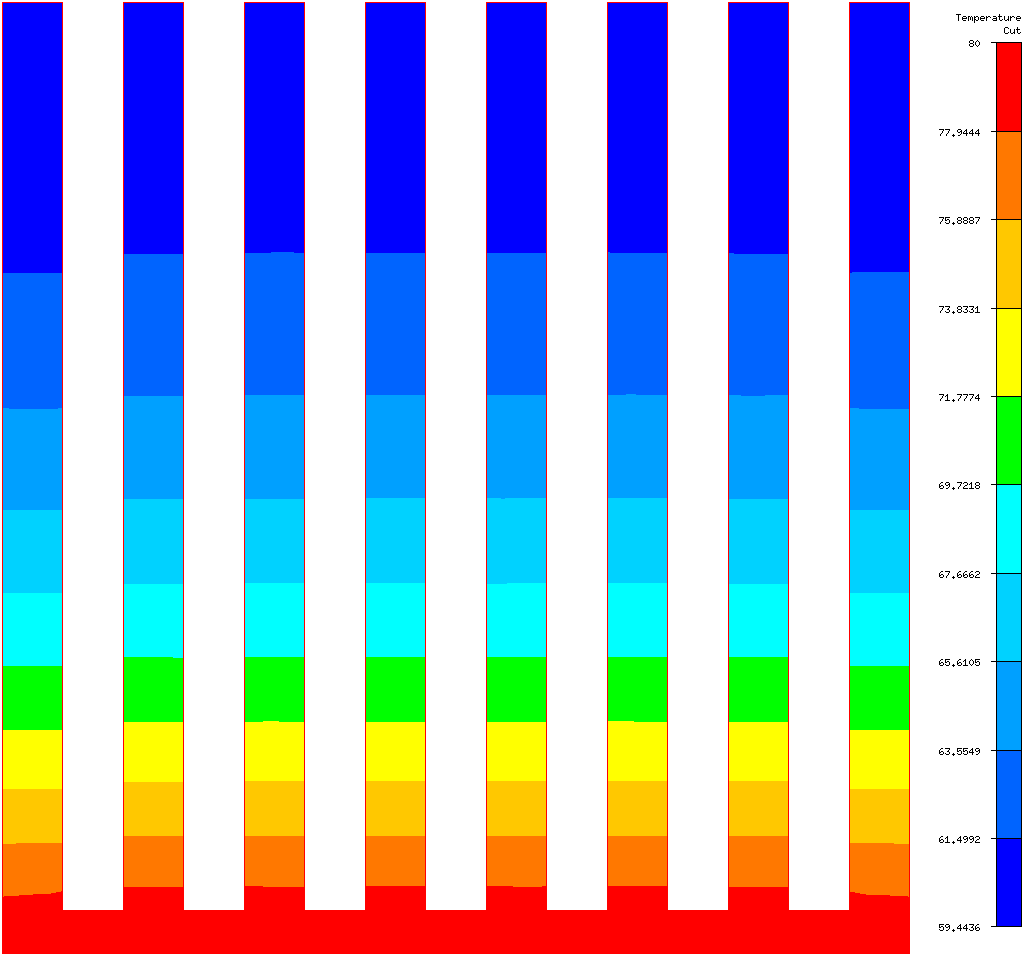
\includegraphics[width=0.7\textwidth]{../figures/heatsink8_h105_gmf005.png}
 \caption{"Placeholder"}
 \label{fig:res_8_1}
 \end{subfigure}
 ~
 \begin{subfigure}[t] {0.23\textwidth}
 \centering
 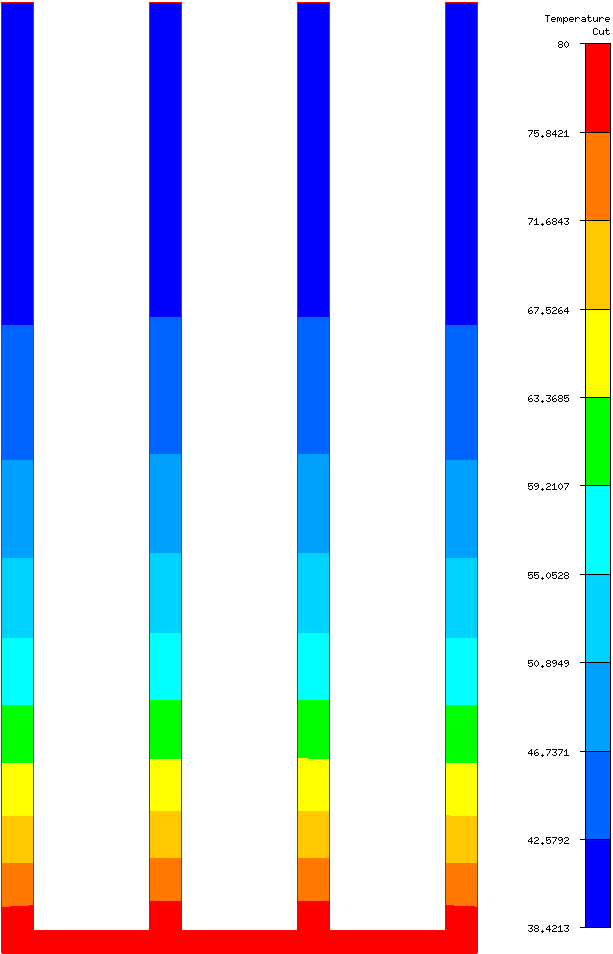
\includegraphics[width=0.7\textwidth]{../figures/heatsink4_h205_gmf005.png}
 \caption{"Placeholder"}
 \label{fig:res_4_2}
 \end{subfigure}
 ~
 \begin{subfigure}[t] {0.23\textwidth}
 \centering
 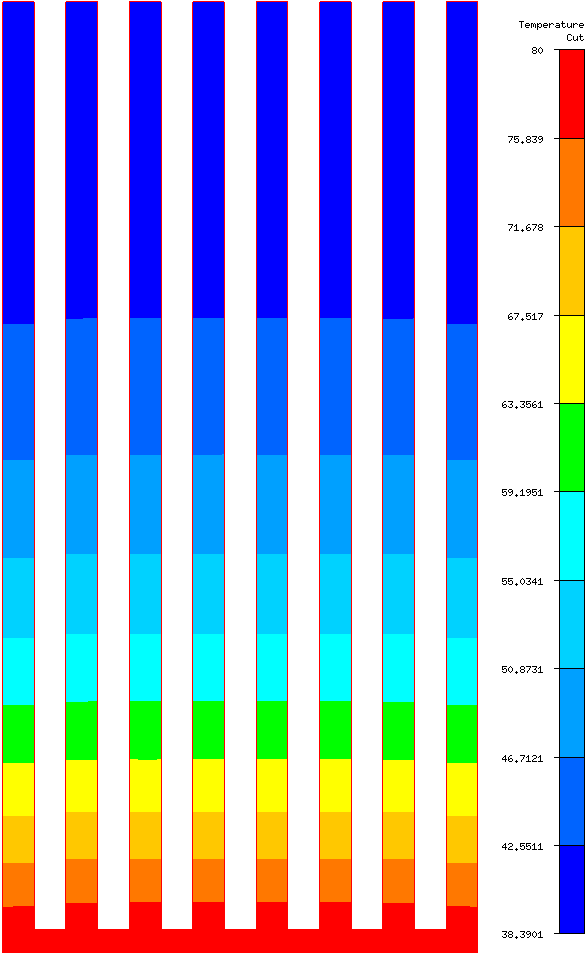
\includegraphics[width=0.7\textwidth]{../figures/heatsink8_h205_gmf005.png}
 \caption{"Placeholder"}
 \label{fig:res_8_2}
 \end{subfigure}
 \caption{These are the different meshes we tried}
 \label{fig:meshes}
 \end{figure}
 
\subsection{Visualization of results}

\subsection{Assumptions and Physical Interpretation}
In our analysis we have made some assumptions and initial choices for the boundary conditions to make a somewhat simplified mathematical model. For the temperature of the bottom of the heat sink base we enforced a constant Dirichlet boundary condition of 80 degrees. This choice was made because it is an estimate of the temperature of a very warm processor working at maximum capacity. By enforcing Dirichlet boundary condition we disallow the hypothetical processor to actually cool down, which is not necessarily a realistic assumption. We would suggest that some kind of Neumann boundary condition would be better suited if you want to see a cooling effect. Another modeling choice made regarding the Robin conditions on the rest of the boundary is that the ambient temperature in the description of the boundary value problem \eqref{eq:heat_bvp} is also constant. This means that even in the tight spaces in between the fins the air temperature is constant. You could think of it as an average temperature on the boundary. One could maybe improve on this assumption by enforcing different ambient temperature on the outer boundary and the boundary in between the fins. Besides you would probably need a very powerful fan to transport the heat away to keep the ambient temperature at 20 degrees as assumed here. 